En este capítulo se expondrán las pruebas experimentales de las principales funcionalidades del paquete, los resultados obtenidos y por supuesto las observaciones de cada prueba de forma separada. Además de un análisis global del comportamiento del paquete para lograr el objetivo señalado en el título de este proyecto.
\section{Calibración y rectificación de las cámaras}
Estas pruebas experimentales buscaban evaluar el funcionamiento de la clase \textbf{StandardStereo} (módulo stereo) hallando los parámetros extrínsecos e intrínsecos de las cámaras. Y comprobando si el algoritmo de rectificación (Ver sección \ref{rectification_section} del capítulo II) posiciona correctamente las disposiciones de las cámaras al mismo tiempo que reduce la distorsión por el tipo de lente empleado.
\\
\\
De acuerdo con la elección realizada en el capítulo IV se seleccionaron las cámaras IMX-219 poseen un FOV de 160$^o$ por lo que en la clase \textbf{StandardStereo} se fijó la variable fish\_eye como verdadera, lo que permitió alcanzar un error RMS inferior a 1 al calibrar y en consecuencia las líneas epipolares en las imágenes rectificadas lograron ser paralelas.
\subsection{Calibración}
\begin{enumerate}
    \item Se ejecutó un servidor local con el Stereopi V2, configurando el sensor de la cámara en 6560 x 2464 píxeles, sin embargo las imágenes reales poseen dimensiones de 3280 x 2464 píxeles, debido a que cada foto tomada por el módulo posee una disposición como la de la Figura \ref{side-by-side} donde en una sola imagen se encuentran ambas escenas, por lo que cada imagen fue recortada por la mitad con la clase \textbf{SplitPair} y reducida a dimensiones de 640 x 720 con el fin de obtener tiempos de procesamiento aceptables.
    \begin{figure}[H]
    \centering
    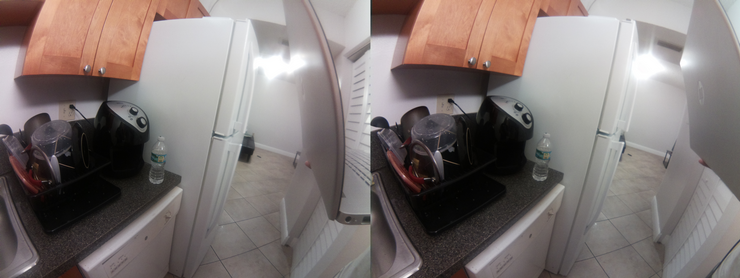
\includegraphics[scale=0.5]{Recursos/side_by_side.png}
    \caption[Disposición de fotos tomadas por StereoPi V2.]{Disposición de fotos tomadas por StereoPi V2. {\footnotesize Fuente: El Autor}}
    \label{side-by-side}
    \end{figure}
    \item Se ejecutaron los pasos de la sección \ref{calibration_section} del capítulo II con 42 imágenes de calibración y con 20, en la tabla \ref{calibration_results} se pueden observar los resultados obtenidos.
    \begin{table}[H]
    \centering
    \caption{Error RMS de calibración}
    \label{calibration_results}
    \begin{tabular}{c|ccc|}
    \cline{2-4}
    \multicolumn{1}{l|}{}                & \multicolumn{3}{c|}{Error}                                                            \\ \hline
    \multicolumn{1}{|c|}{$N^o$ imágenes} & \multicolumn{1}{c|}{cámara izquierda} & \multicolumn{1}{c|}{cámara derecha} & estéreo \\ \hline
    \multicolumn{1}{|c|}{42}             & \multicolumn{1}{c|}{0.31}             & \multicolumn{1}{c|}{0.19}           & 0.28    \\ \hline
    \multicolumn{1}{|c|}{20}             & \multicolumn{1}{c|}{0.20}             & \multicolumn{1}{c|}{0.19}           & 0.21    \\ \hline
    \end{tabular}
    \end{table}
\end{enumerate}
\subsection{Rectificación}
En la Figura \ref{rectification_result} se puede apreciar el efecto de la rectificación.
\begin{figure}[H]
    \centering
    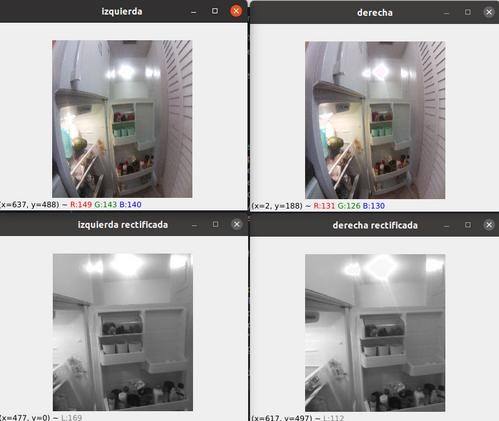
\includegraphics[scale=0.6]{Recursos/rectification_result.jpg}
    \caption[Efecto de la rectificación.]{Efecto de la rectificación. {\footnotesize Fuente: El Autor}}
    \label{rectification_result}
\end{figure}
Para verificar la calidad de la rectificación en los dos casos expuestos de la tabla \ref{calibration_results} se dibujaron las líneas epipolares con el método find\_epilines, el cual pertenece a la clase \textbf{StandardStereoBuilder} obteniendo así las Figuras \ref{epilines_20} y \ref{epilines_42}
\begin{figure}[H]
    \centering
    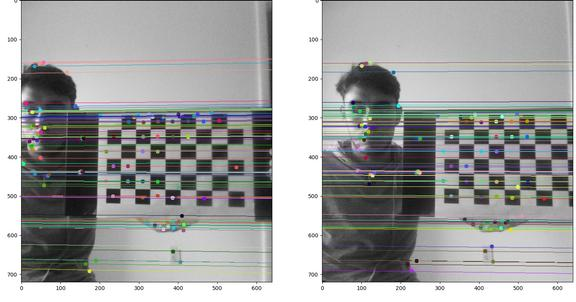
\includegraphics[scale=0.4]{Recursos/epilines_20_calibration_images.jpg}
    \caption[Líneas epipolares para 20 imágenes de calibración.]{Líneas epipolares para 20 imágenes de calibración. {\footnotesize Fuente: El Autor}}
    \label{epilines_20}
\end{figure}
\begin{figure}[H]
    \centering
    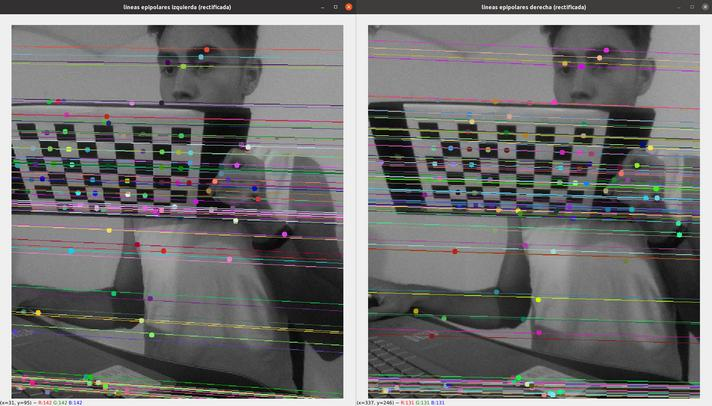
\includegraphics[scale=0.3]{Recursos/epilines_42_calibration_images.jpg}
    \caption[Líneas epipolares para 42 imágenes de calibración.]{Líneas epipolares para 42 imágenes de calibración. {\footnotesize Fuente: El Autor}}
    \label{epilines_42}
\end{figure}
\subsection{Análisis de resultados}
Como se puede observar en la tabla \ref{calibration_results} el número propuesto por Zhengyou Zhang \cite{Zhang2000} es acertado, puesto que la calibración es un método iterativo, demasiadas imágenes pueden llegar a ser contraproducente, debido a que el error termina divergiendo y en lugar de reducirse comienza a aumentar, esto se termina de comprobar en las Figuras \ref{epilines_20} y \ref{epilines_42}, donde a pesar de que en ambas imágenes dichas líneas son paralelas precisamente la que utiliza 20 imágenes logra un mejor resultado que permite reducir verdaderamente el problema de correspondencia, cabe resaltar que a pesar de reducir las dimensiones de las imágenes de entrada, esto no afecta en el cálculo de los parámetros de las cámaras y del sistema estéreo en sí, incluso es posible ingresar otras dimensiones en el paso de rectificación en caso de ser necesario. 
\\
\\
Adicionalmente se logra apreciar que el proceso de rectificación fue satisfactorio, porque las imágenes de muestra en la Figura \ref{rectification_result} eliminan las distorsiones causadas por las cualidades de las cámaras y especialmente el efecto de distorsión radial del lente.
\section{Cálculo de disparidad}
El objetivo de esta prueba experimental es comprobar que el algoritmo estéreo implementado en el módulo stereo funcione correctamente, además de ajustar varias configuraciones de los parámetros propios del algoritmo SGBM, de tal forma que se obtengan mapas de disparidad acordes con la realidad, por medio del algoritmo dentro del archivo stereo\_tuner.py en la carpeta tutorials. Adicionalmente se busco comprobar el efecto del paso de post-procesamiento en cuanto a calidad de mapa de disparidad y tiempo de ejecución.
\\
\\
Para lograrlo se captaron 9 imágenes en un entorno cerrado y 2 en un entorno abierto (redimensionadas a 640 x 720 píxeles) bajo diferentes perspectivas para observar el comportamiento de los mapas de disparidad ante los ajustes de los parámetros del algoritmo estéreo SGBM, dichas imágenes se pueden encontrar en el repositorio de github del paquete.
\subsection{Ajuste de parámetros}
Se creó un script para el ajuste de los parámetros del algoritmo estéreo, dicho archivo se encuentra en el repositorio https://github.com/corvus96/PyTwoVision dentro de la carpeta tutorials. Se seleccionaron 3 conjuntos de ajustes los cuales se pueden observar en la tabla \ref{tune_parameters}
\begin{table}[H]
\centering
\caption{Ajuste de valores algoritmo de correspondencia}
\label{tune_parameters}
\begin{tabular}{|c|ccc|}
\hline
                             & \multicolumn{3}{c|}{Configuraciones}                                                    \\ \hline
Parámetros                   & \multicolumn{1}{c|}{A}             & \multicolumn{1}{c|}{B}             & M             \\ \hline
Disparidad mínima            & \multicolumn{1}{c|}{-32}           & \multicolumn{1}{c|}{-33}           & -32           \\ \hline
Número de disparidades       & \multicolumn{1}{c|}{32}            & \multicolumn{1}{c|}{32}            & 32            \\ \hline
Tamaño de bloque             & \multicolumn{1}{c|}{3}             & \multicolumn{1}{c|}{3}             & 3             \\ \hline
Disp12MaxDiff                & \multicolumn{1}{c|}{-38}           & \multicolumn{1}{c|}{-38}            & -38            \\ \hline
Rango de motas               & \multicolumn{1}{c|}{1}             & \multicolumn{1}{c|}{9}             & 5             \\ \hline
Tamaño de la ventana moteada & \multicolumn{1}{c|}{114}           & \multicolumn{1}{c|}{120}           & 117           \\ \hline
P1                           & \multicolumn{1}{c|}{89}           & \multicolumn{1}{c|}{125}            & 107           \\ \hline
P2                           & \multicolumn{1}{c|}{487}          & \multicolumn{1}{c|}{932}          & 710          \\ \hline
Relación de unicidad         & \multicolumn{1}{c|}{3}             & \multicolumn{1}{c|}{3}             & 3             \\ \hline
modo                         & \multicolumn{1}{c|}{8 direcciones} & \multicolumn{1}{c|}{8 direcciones} & 8 direcciones \\ \hline
Pre-filter cap               & \multicolumn{1}{c|}{14}            & \multicolumn{1}{c|}{57}            & 36            \\ \hline
Lambda                       & \multicolumn{1}{c|}{8214}         & \multicolumn{1}{c|}{19132}         & 13673         \\ \hline
Sigma                        & \multicolumn{1}{c|}{1.589}         & \multicolumn{1}{c|}{1.046}          & 1.318         \\ \hline
\end{tabular}
\end{table}
A continuación se presentarán los mapas de disparidad para las 3 configuraciones sin aplicar el paso de post-procesamiento:
\begin{figure}[H]
    \centering
    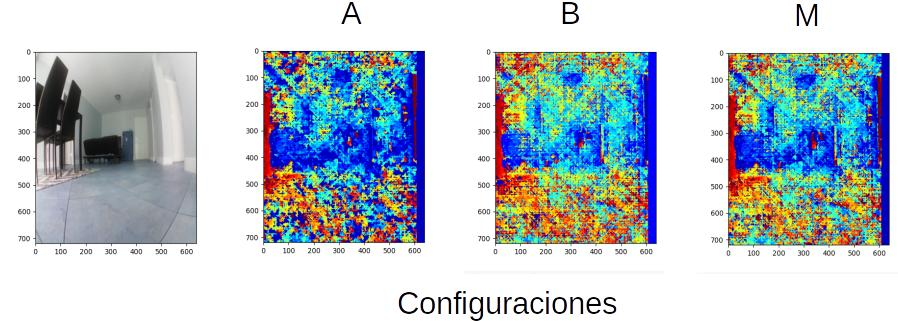
\includegraphics[scale=0.6]{Recursos/disparity_maps_without_postprocessing_results.jpg}
    \caption[Mapas de disparidad para las 3 configuraciones sin post-procesamiento.]{Mapas de disparidad para las 3 configuraciones sin post-procesamiento. {\footnotesize Fuente: El Autor}}
    \label{disparity_without_postprocess}
\end{figure}
Y aplicando post-procesamiento:
\begin{figure}[H]
    \centering
    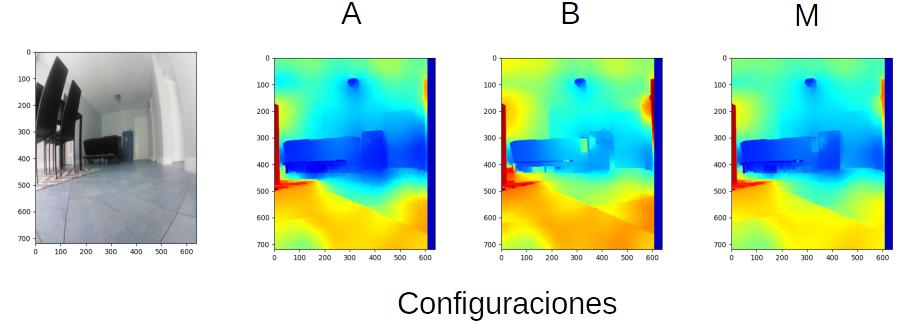
\includegraphics[scale=0.6]{Recursos/disparity_maps_with_postprocessing_results.jpg}
    \caption[Mapas de disparidad para las 3 configuraciones con post-procesamiento.]{Mapas de disparidad para las 3 configuraciones con post-procesamiento. {\footnotesize Fuente: El Autor}}
    \label{disparity_with_postprocess}
\end{figure}
\subsection{Tiempo de ejecución}
Dado que el código estéreo no utiliza procesamiento paralelo, hecho que se comprobó ejecutándolo en la plataforma de Google Colab obteniendo resultados similares a los alcanzados en el computador local, se obtuvo la velocidad de procesamiento de la etapa de correspondencia y de post-procesamiento en el computador local, al aplicar un redimensionamiento en las imágenes rectificadas, por lo que en la tabla \ref{speed_matching_results} se pueden observar los valores obtenidos.
\begin{table}[H]
\caption{Efecto del redimensionamiento en la velocidad del proceso estéreo}
\label{speed_matching_results}
\begin{tabular}{|cc|c}
\cline{1-2}
\multicolumn{2}{|c|}{Tiempo de ejecución de etapa}         &                                           \\ \hline
\multicolumn{1}{|c|}{correspondencia} & post-procesamiento & \multicolumn{1}{c|}{factor de escala} \\ \hline
\multicolumn{1}{|c|}{0.1691}          & 0.0249             & \multicolumn{1}{c|}{1}                    \\ \hline
\multicolumn{1}{|c|}{0.0374}          & 0.0034             & \multicolumn{1}{c|}{1/2}                  \\ \hline
\multicolumn{1}{|c|}{0.0090}          & 0.0022             & \multicolumn{1}{c|}{1/4}                  \\ \hline
\multicolumn{1}{|c|}{0.0024}          & 0.0017             & \multicolumn{1}{c|}{1/8}                  \\ \hline
\end{tabular}
\end{table}
Es importante recalcar que el ajuste de dimensiones aplicado, corresponde con el mencionado en el paso de preprocesamiento, por lo que el ancho y alto nuevo serán $ancho\cdot factor$ y $alto\cdot factor$ de modo que la imagen pre-procesada tendrá 1/4 de la dimensión original en el caso de ser 1/2.
\subsection{Análisis de resultados}
Al comparar las Figuras \ref{disparity_without_postprocess} y \ref{disparity_with_postprocess} se observa que efectivamente el paso de post-procesamiento mejora notablemente la calidad de los mapas de disparidad y su tiempo de ejecución es entre un 10\% a 20\% la duración del paso de correspondencia, el ajuste de parámetros es una tarea que requiere iterar constantemente hasta conseguir los mejores resultados posibles, en este caso se ajustaron primero los casos A y B, mientras que la configuración M surgió de hallar el valor promedio entre los parámetros de A y B. 
\\
\\
Por otro lado en la tabla \ref{speed_matching_results} se aprecia como claramente la reducción de las imágenes rectificadas tiene un efecto considerable en el tiempo de ejecución, sin olvidar que estos tiempos están asociados al procesador utilizado. A pesar de ello, no se debe abusar de la reducción de tamaño, porque si bien es cierto que el método usado para redimensionar logra recuperar más información que un método convencional, al recuperar el tamaño original de una imagen la cual fue reducida con un factor de escala por encima de un 1/4 pueden ocurrir dos cosas:
\begin{itemize}
    \item Si la imagen rectificada se encontraba desplazada al menos unos píxeles, es decir que existiese una banda vertical en los laterales de la imagen, la imagen final tendría las mismas bandas, pero con un mayor grosor, lo que reduciría el campo de visión.
    \item Los detalles u objetos pequeños del mapa de disparidad podrían verse eliminados.
\end{itemize}
No obstante, el límite de factor de escala dependerá del tamaño de las imágenes de entrada.
\section{Entrenamiento de YOLO V3}
Esta prueba experimental verifica el rendimiento de todo el proceso de entrenamiento y evaluación de una red YOLO V3 utilizando las clases propuestas en el módulo recognition.
\\
\\
Para realizar el entrenamiento se utilizó la plataforma de Google Colab y las gráficas que representan la evolución de la red en el entrenamiento fueron generadas con Tensorboard (herramienta de Tensorflow).
\subsection{Conjunto de datos}
Se seleccionó el conjunto de datos PASCAL VOC 2012 \cite{pascal-voc-2012}, el cual cuenta con 20 clases repartidas en 17125 imágenes, dicho conjunto fue dividido de forma aleatoria en datos de entrenamiento asignándole el 80\% (13700) y datos de validación con el 20\% restante (3425).
\subsection{Hiperparámetros}
\begin{itemize}
    \item warmup\_epochs = 5
    \item lr\_init = $10^{-3}$
    \item lr\_end = $10^{-6}$
    \item batch\_size = 20, a consecuencia de este tamaño de lote dado que en una iteración son introducidas 20 imágenes a la red, para completar un \textit{epoch} se necesitaron 685 iteraciones.
    \item \textit{epochs} = 160, sin embargo se detuvo el entrenamiento en el número 75 en vista de que el error de validación comenzaba a subir en lugar de bajar desde el \textit{epoch} número 37.
\end{itemize}
Para el resto de los hiperparámetros se seleccionaron las opciones por defecto. 
\subsection{Rutina de entrenamiento/validación}
El tiempo de entrenamiento fue de 19.28 horas, no obstante el mejor resultado fue alcanzado en el \textit{epoch} número 37, a las 9.50 horas, este hecho se puede observar claramente en la Figura \ref{validation_result} donde se alcanza el punto de inflexión precisamente en dicho epoch (iteración número 25354), cabe resaltar que a pesar de que el error de entrenamiento continúa descendiendo (Ver Figura \ref{training_result}) luego de dicho número de iteraciones, por norma cuando el error de validación comienza a subir la red tiende a sufrir de \textit{overfitting} (sobre ajuste).
\begin{figure}[H]
    \centering
    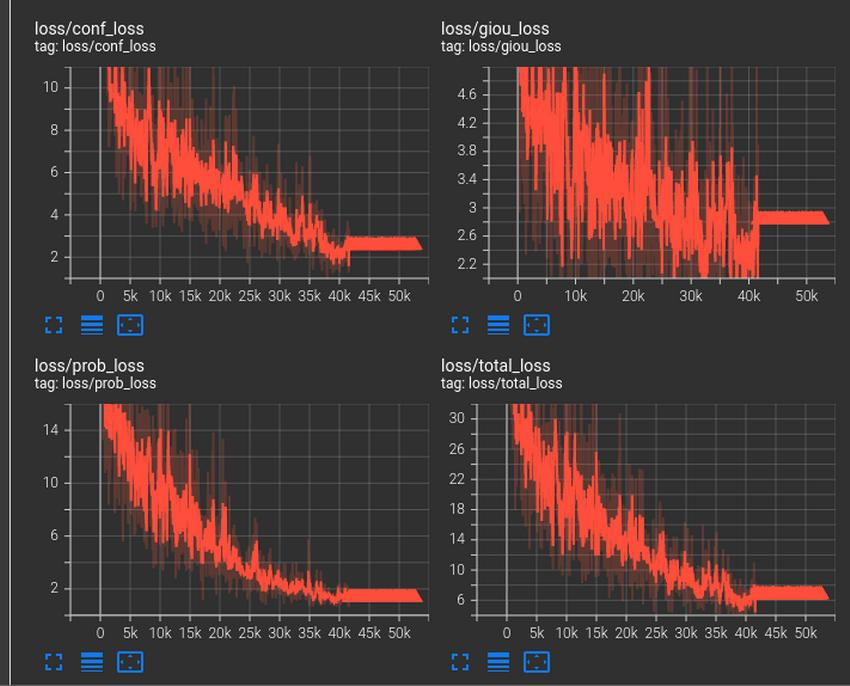
\includegraphics[scale=0.4]{Recursos/training_loss_result.jpg}
    \caption[Errores de entrenamiento (Error vs. Número de iteración).]{Errores de entrenamiento (Error vs. Número de iteración). {\footnotesize Fuente: El Autor}}
    \label{training_result}
\end{figure}
\begin{figure}[H]
    \centering
    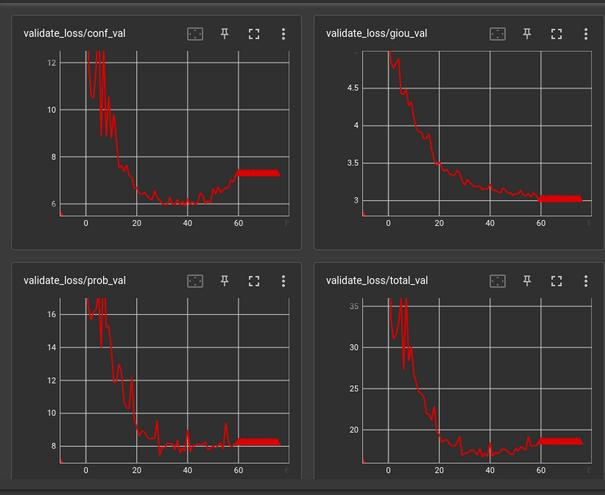
\includegraphics[scale=0.6]{Recursos/validation_loss_result.jpg}
    \caption[Errores de validación (Error vs. Número de \textit{epoch}).]{Errores de validación (Error vs. Número de \textit{epoch}). {\footnotesize Fuente: El Autor}}
    \label{validation_result}
\end{figure}
En la Figura \ref{learning_rate_result} se observa como el \textit{learning rate} evoluciono con cada iteración y efectivamente este cumple la regla impuesta por el warmup\_epochs de crecer linealmente durante 5 \textit{epochs} (3425 iteraciones) y comenzar a decaer luego de dicho límite.
\begin{figure}[H]
    \centering
    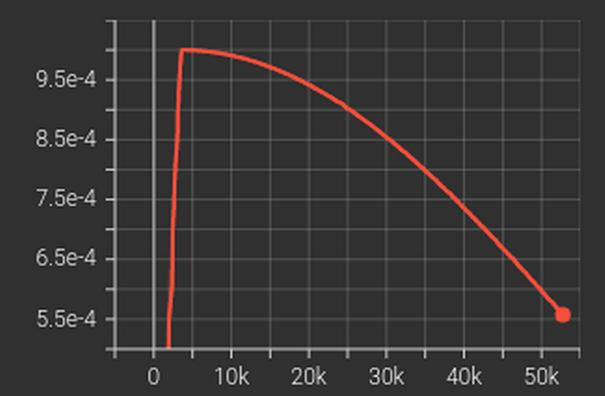
\includegraphics[scale=0.6]{Recursos/learning_rate_evolution_result.jpg}
    \caption[Evolución del \textit{learning rate} vs. Número de iteración).]{Evolución del \textit{learning rate} vs. Número de iteración). {\footnotesize Fuente: El Autor}}
    \label{learning_rate_result}
\end{figure}
Es menester resaltar que el error de validación alcanzado en el \textit{epoch} 37 es:
\begin{itemize}
    \item error de clasificación o probabilidad = 7.60 \%.
    \item error de confianza = 5.95 \%.
    \item error por GIoU = 3.14 \%.
\end{itemize}
Por lo que el error total es de 16.69 \%.
\subsection{Evaluación}
En las Figuras \ref{mAP_50_result}, \ref{mAP_75_result}, \ref{mAP_100_result}, se aprecia el cálculo de la métrica mAP para cada clase y el total, como era de esperar a medida que el umbral se eleva el resultado final disminuye.
\begin{figure}[H]
     \centering
     \begin{subfigure}[b]{0.4\textwidth}
        \centering
        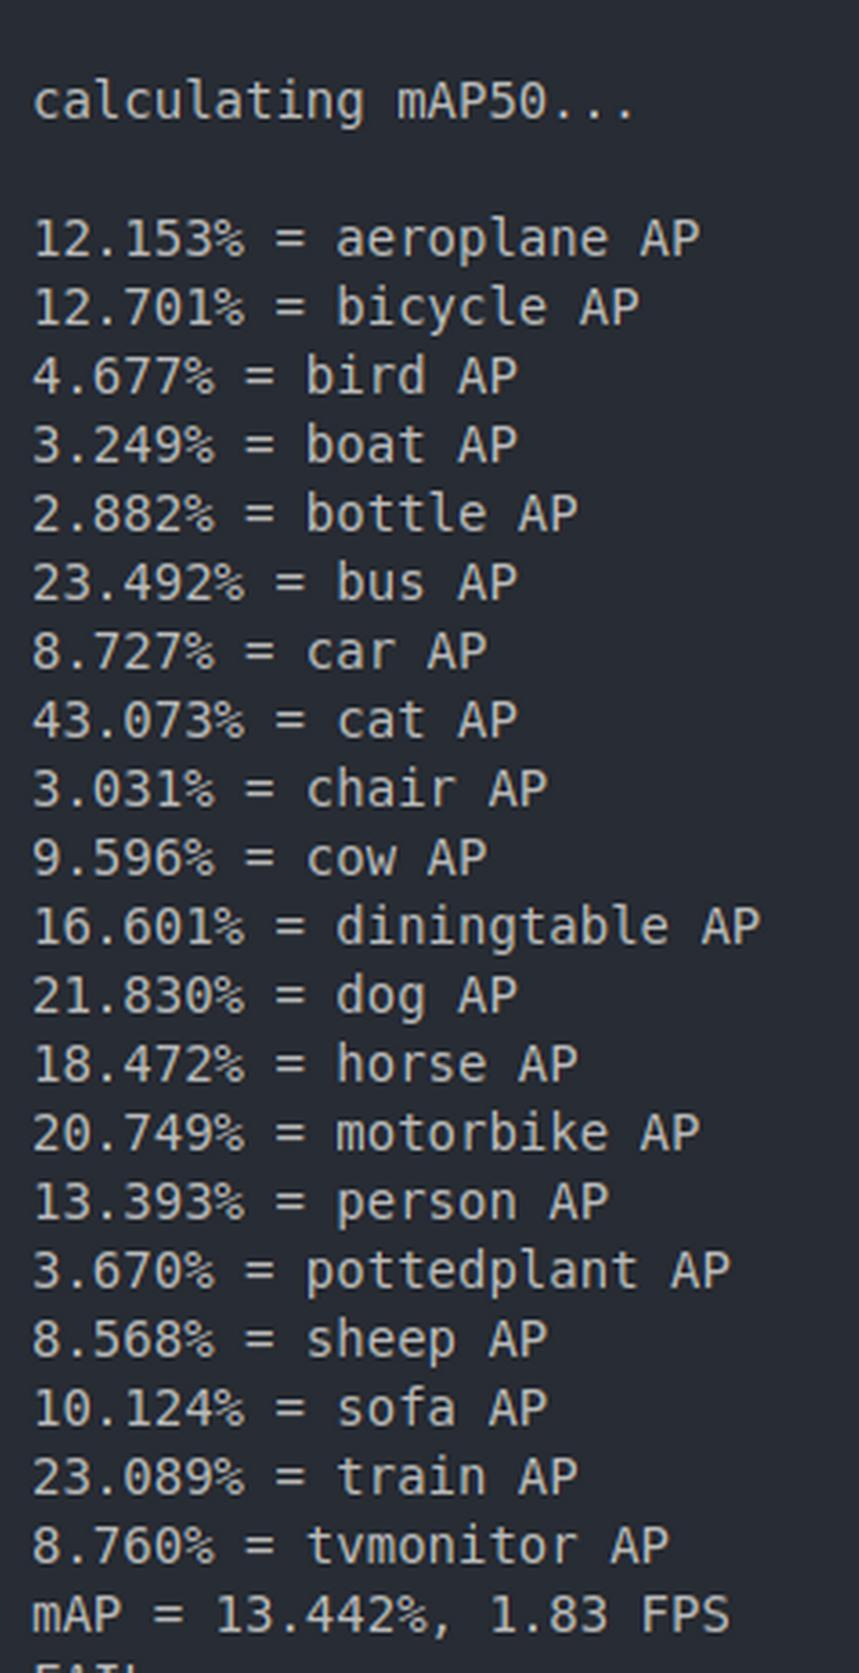
\includegraphics[scale=0.15]{Recursos/mAP50_result.jpg}
        \caption[$mAP_{50}$.]{$mAP_{50}$. {\footnotesize Fuente: El Autor}}
        \label{mAP_50_result}
     \end{subfigure}
     \hfill
     \begin{subfigure}[b]{0.4\textwidth}
         \centering
        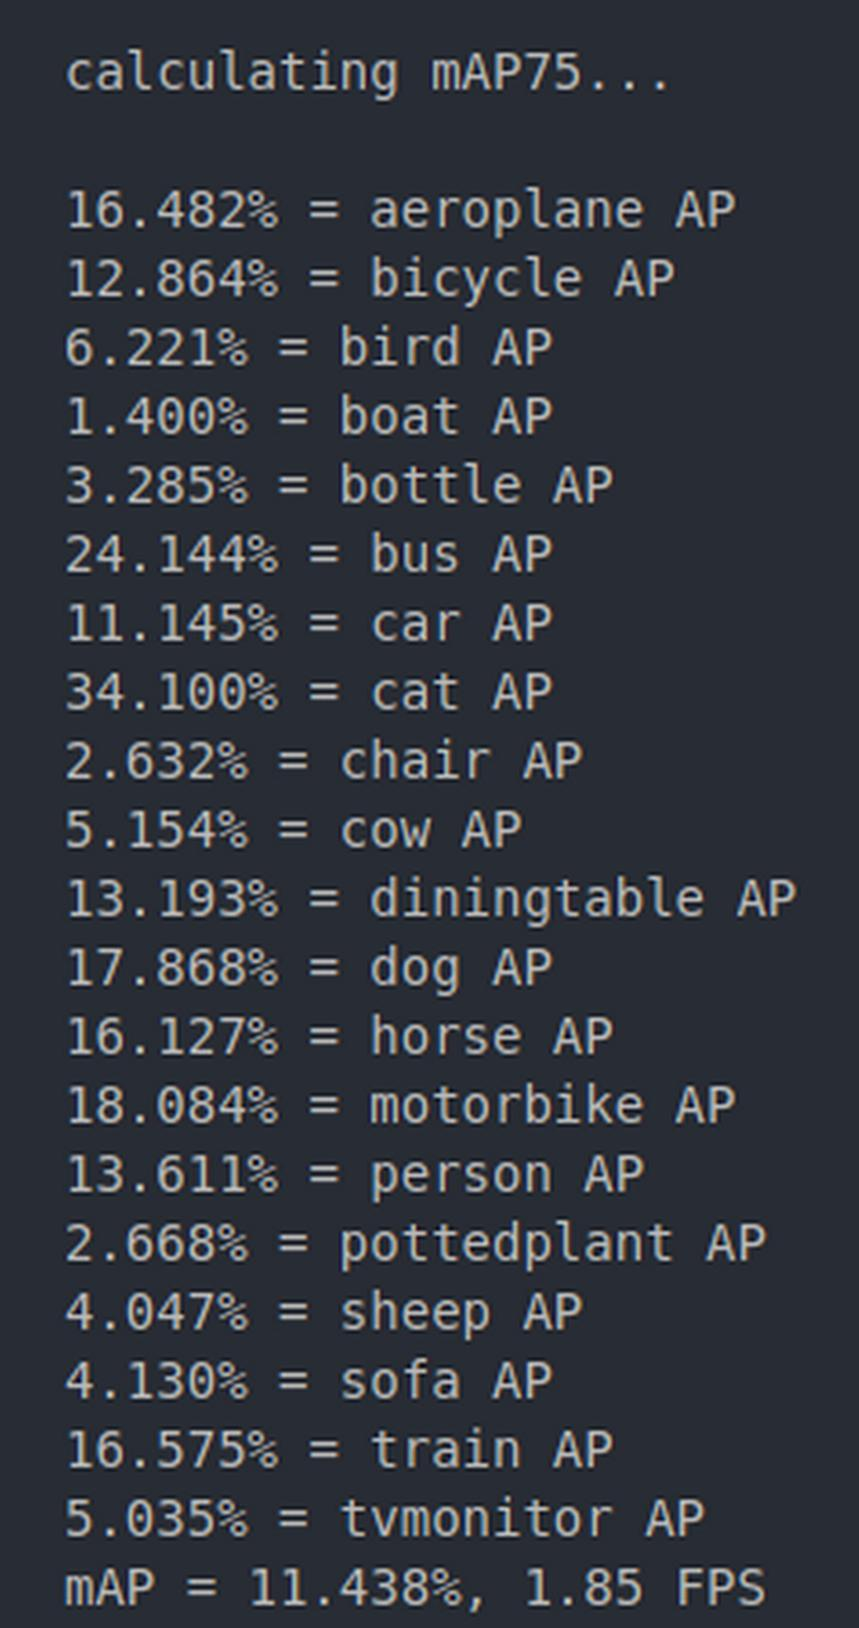
\includegraphics[scale=0.15]{Recursos/mAP75_result.jpg}
        \caption[$mAP_{75}$.]{$mAP_{75}$. {\footnotesize Fuente: El Autor}}
        \label{mAP_75_result}
     \end{subfigure}
     \hfill
     \begin{subfigure}[b]{0.4\textwidth}
         \centering
        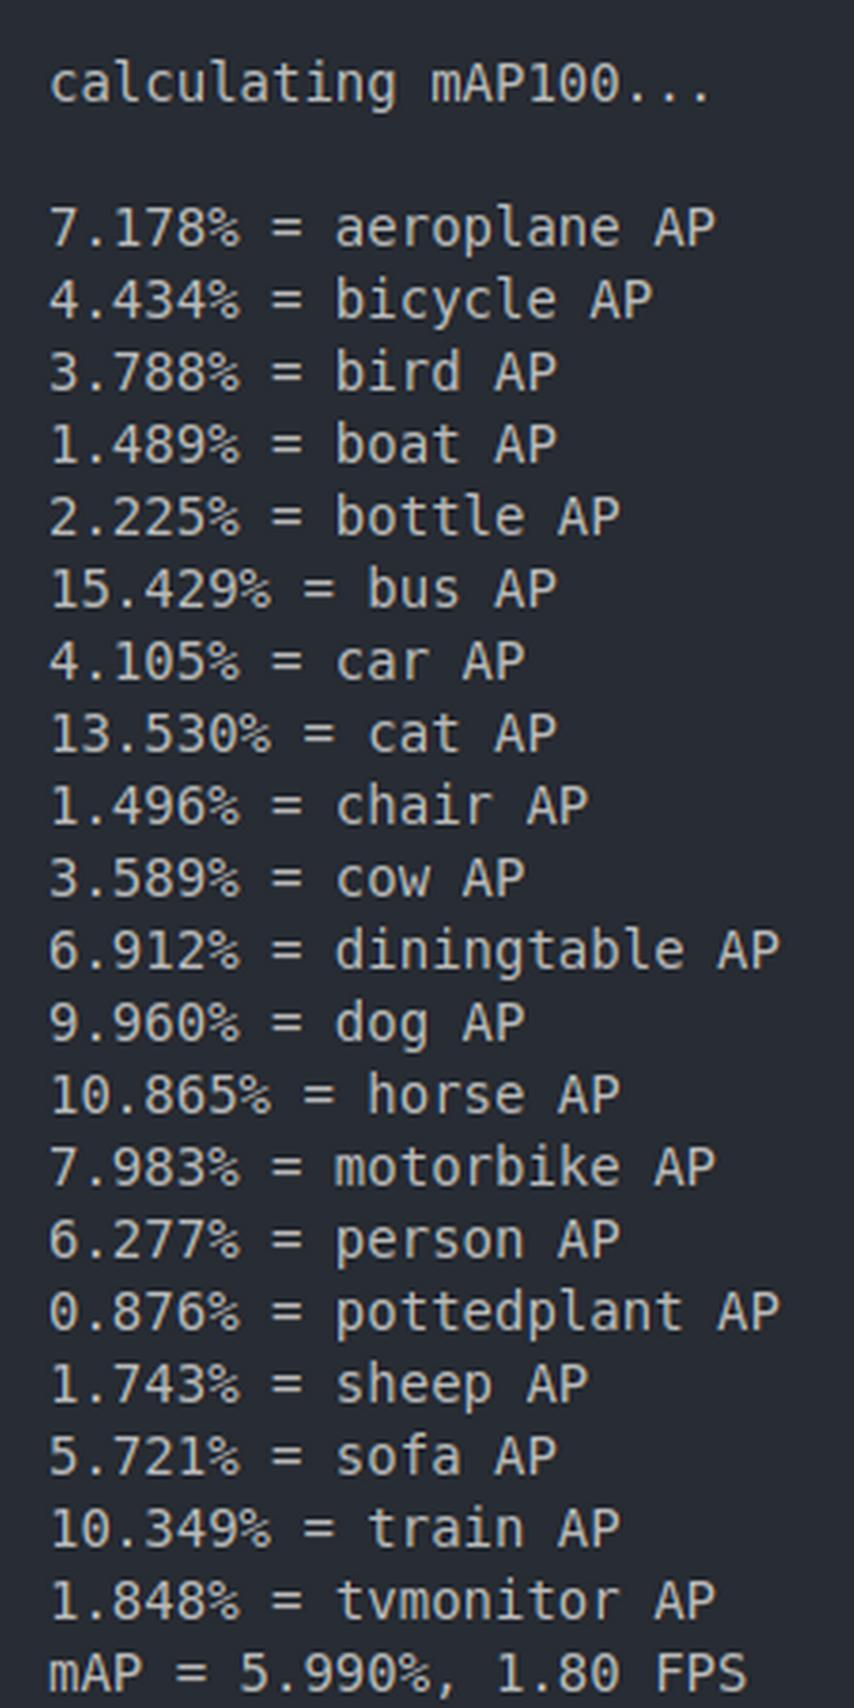
\includegraphics[scale=0.15]{Recursos/mAP100_result.jpg}
        \caption[$mAP_{100}$.]{$mAP_{100}$. {\footnotesize Fuente: El Autor}}
        \label{mAP_100_result}
     \end{subfigure}
\caption{\textit{Mean Average precision} (mAP) para distintos umbrales}
\label{mAP_results}
\end{figure}
\subsection{Tiempo de ejecución}
Se evaluó dicho tiempo tanto para el computador local como en el servidor de Google Colab, obteniendo aproximadamente 1.8 \textit{frames} por segundo (555.56 ms) en el computador local y 12.36 FPS (80.91 ms) en la plataforma de Colab cuando se utiliza la GPU.
\subsection{Análisis de resultados}
Es notable que aunque el error de validación se encuentre por encima del valor recomendable que debería ser por debajo del 1\%, aun así el modelo es capaz de obtener resultados aceptables para inferir en un ambiente cerrado con buena iluminación, como se puede ver en la Figura \ref{training_result} los errores de entrenamiento se mantienen siempre por debajo de los de validación, esto se debe a que cuando se realiza la validación, la red no está ajustando los pesos, ya que solo está comprobando el entrenamiento al introducir nuevos datos, por este motivo se trata de evitar el \textit{overfitting} dividiendo el conjunto de datos, con el fin de que la red pueda generalizar de mejor manera.
\\
\\
Además en las Figuras \ref{training_result} y \ref{validation_result} se observa ruido (el error es infinito) después del \textit{epoch} 60 esto se debe a que en ese punto se desconectó la máquina virtual de Colab y al volver a conectar la red continuó el entrenamiento con los mismos pesos, pero aplicando la estrategia de \textit{warmup} partiendo con el mínimo \textit{learning rate} posible, esto en sí mismo es un error debido a que cuando se tienen pesos ya entrenados la etapa de \textit{warmup} de 5 \textit{epochs} en este caso es innecesaria, lo correcto seria entrenar con un \textit{warmup} de 0.
\\
\\
Otro motivo por el que puede que la red no sea capaz de mejorar sus resultados, es debido a que varios autores recomiendan al menos 1000 imágenes por clase, para conseguir una buena generalización, sin embargo; para esto la red debería tener al menos 20000 imágenes, una solución a esto podría ser tomar pesos ya entrenados y aplicar transferencia de aprendizaje. En cuanto a la velocidad de la red el tiempo de predicción se reduce significativamente con el uso de una GPU dedicada como la de Colab.
\section{Posicionamiento}
En estas pruebas se tiene como objetivos comprobar el funcionamiento de la umbralización de Otsu en una ventana de detección y hallar el error absoluto promedio entre la posición real de la coordenada Z de un objeto y su posición calculada mediante el módulo input\_output.
\\
\\
Para estas pruebas se emplearon las configuraciones A, B y M de los mapas de correspondencia y se cargaron los pesos del conjunto de datos COCO con el método restore\_weights de la clase Recognizer. COCO cuenta con 80 clases y más de 200 mil imágenes, su mayor variedad de objetos y mejor precisión fue la razón de su elección para comprobar la ubicación de objetos de diferentes características.
\subsection{Efecto de umbralización de Otsu}
Uno de los pilares de la metodología de posicionamiento es la segmentación por umbralización de Otsu y a pesar de que no es perfecta, dadas las condiciones impuestas, es posible obtener resultados favorables, tal es el caso de la Figura \ref{otsu_bike}, que aunque tiene una línea de píxeles que no corresponden con el objeto detectado, la mayoría de ellos si pertenecen a dicho objeto y dado que la posición es la media de las coordenadas de todos esos píxeles, la distancia tiende a ser la del objeto en sí mismo y no la del fondo de su \textit{bounding box}. 
\\
\\
No obstante, hay casos en los que no siempre funciona adecuadamente como se puede ver en la Figura \ref{otsu_inverso} que en lugar de segmentar la botella de plástico sucede lo contrario esto es debido a que este método en su versión inversa favorece los píxeles más oscuros, por este motivo para tratar con ese tipo de objetos se agregó una variable booleana que permite alternar entre la umbralización inversa y normal, la segunda favorece a píxeles más cercanos al blanco y es bastante preciso en segmentar botellas transparentes como es el caso de la Figura \ref{otsu_normal}.
\begin{figure}[H]
     \centering
     \begin{subfigure}[b]{0.4\textwidth}
        \centering
        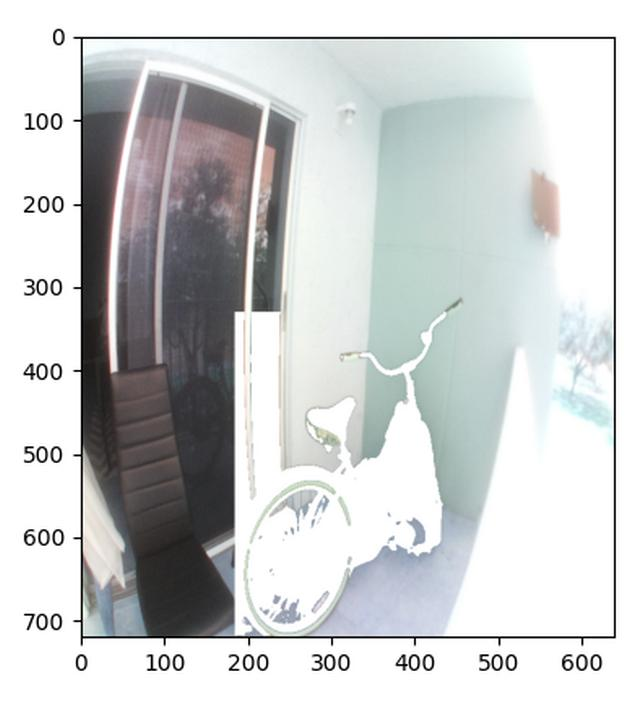
\includegraphics[scale=0.35]{Recursos/otsu_bike.jpg}
        \caption[Umbralización en una bicicleta.]{Umbralización en una bicicleta. {\footnotesize Fuente: El Autor}}
        \label{otsu_bike}
     \end{subfigure}
     \hfill
     \begin{subfigure}[b]{0.4\textwidth}
        \centering
        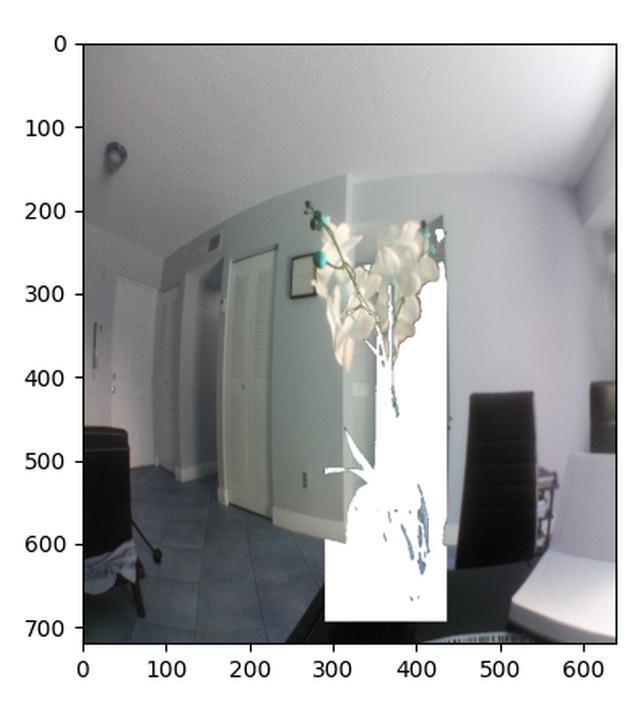
\includegraphics[scale=0.35]{Recursos/otsu_position.jpg}
        \caption[Umbralización en una flor.]{Umbralización en una flor. {\footnotesize Fuente: El Autor}}
        \label{otsu_position}
     \end{subfigure}
     \hfill
     \begin{subfigure}[b]{0.4\textwidth}
        \centering
        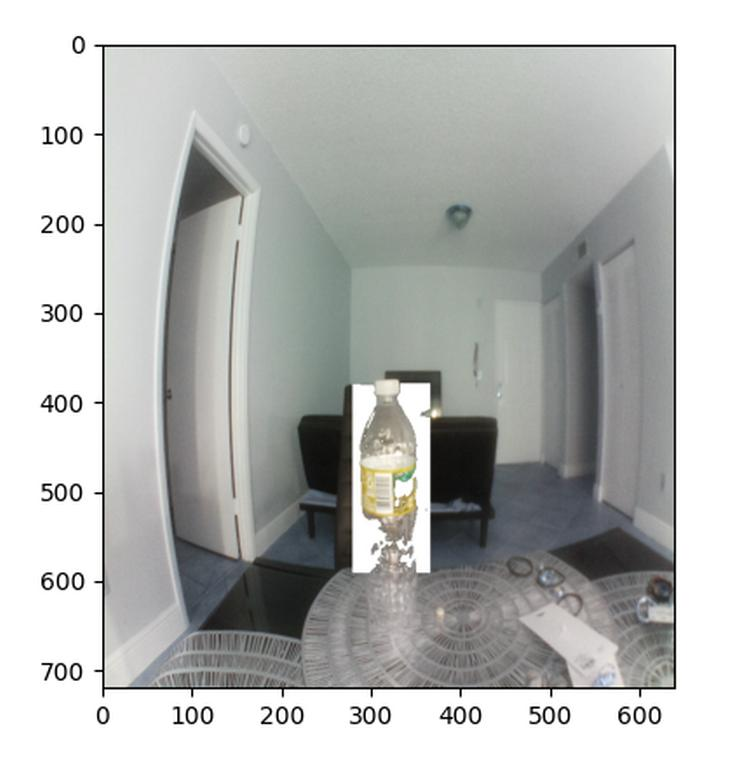
\includegraphics[scale=0.35]{Recursos/umbral_inverso.jpg}
        \caption[Umbralización inversa.]{Umbralización inversa. {\footnotesize Fuente: El Autor}}
        \label{otsu_inverso}
     \end{subfigure}
     \hfill
     \begin{subfigure}[b]{0.4\textwidth}
         \centering
        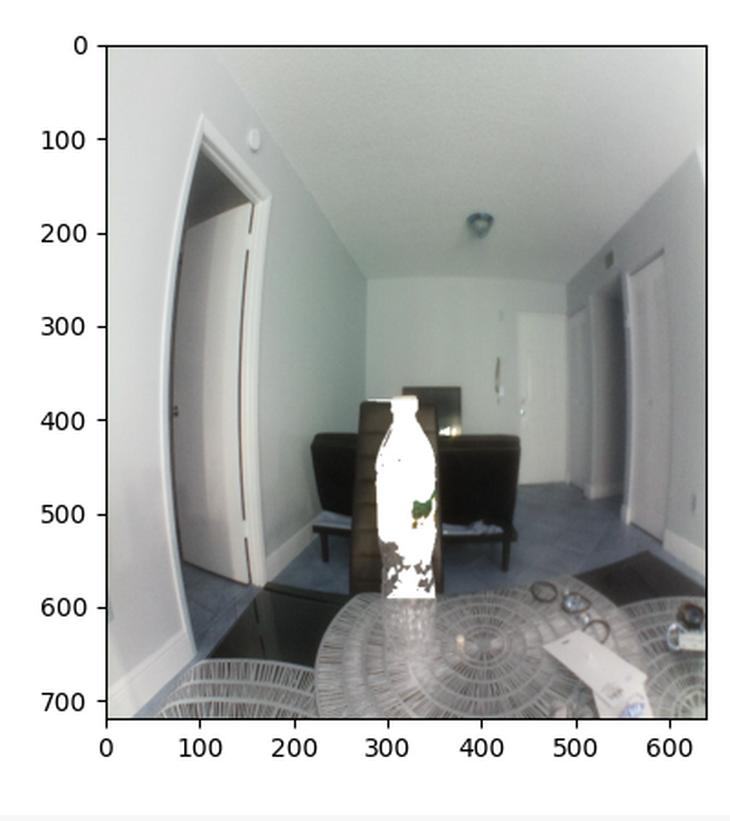
\includegraphics[scale=0.31]{Recursos/umbral_normal.jpg}
        \caption[Umbralización normal.]{Umbralización normal. {\footnotesize Fuente: El Autor}}
        \label{otsu_normal}
     \end{subfigure}
\caption{Segmentación binaria de Otsu}
\label{OTSU_segmentation}
\end{figure}
Para las pruebas realizadas a continuación se eligió la versión inversa debido a que es más probable que los objetos detectados se encuentren superpuestos a su fondo y por ende sus píxeles sean más oscuros.
\subsection{Posición real vs. configuraciones A, B y M}
Para convertir los mapas de disparidad en distancia se usó la siguiente matriz Q:
\begin{align}
    Q = \begin{bmatrix}
            1 & 0 & 0 & -320\\
            0 & 1 & 0 & -360\\
            0 & 0 & 0 & 309\\
            0 & 0 & -1.5385 & 0
            \end{bmatrix}
\end{align}
Donde el valor de la distancia focal fue extraído de la matriz de la cámara y la línea base fue medida directamente en el sistema.
\\
\\
Se tomó como elemento de prueba la flor de la imagen \ref{otsu_position}, la cual se encuentra a una distancia de $0.35 \pm 0.01$ m del sistema estéreo y se generaron las Figuras \ref{pos_conf_A}, \ref{pos_conf_B} y \ref{pos_conf_M}, cuyas coordenadas se encuentran en la escala de metros.
\begin{figure}[H]
    \centering
    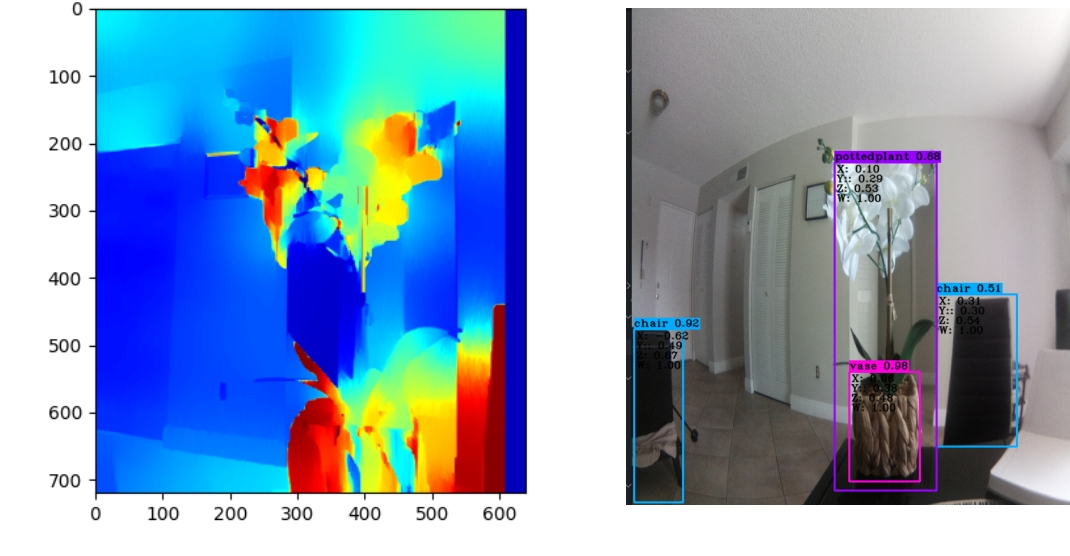
\includegraphics[scale=0.5]{Recursos/position_configuration_A.jpg}
    \caption[Mapa de disparidad y coordenadas con configuración A.]{Mapa de disparidad y coordenadas con configuración A. {\footnotesize Fuente: El Autor}}
    \label{pos_conf_A}
\end{figure}
El error absoluto del objeto para la configuración A es de 0.18
\begin{figure}[H]
    \centering
    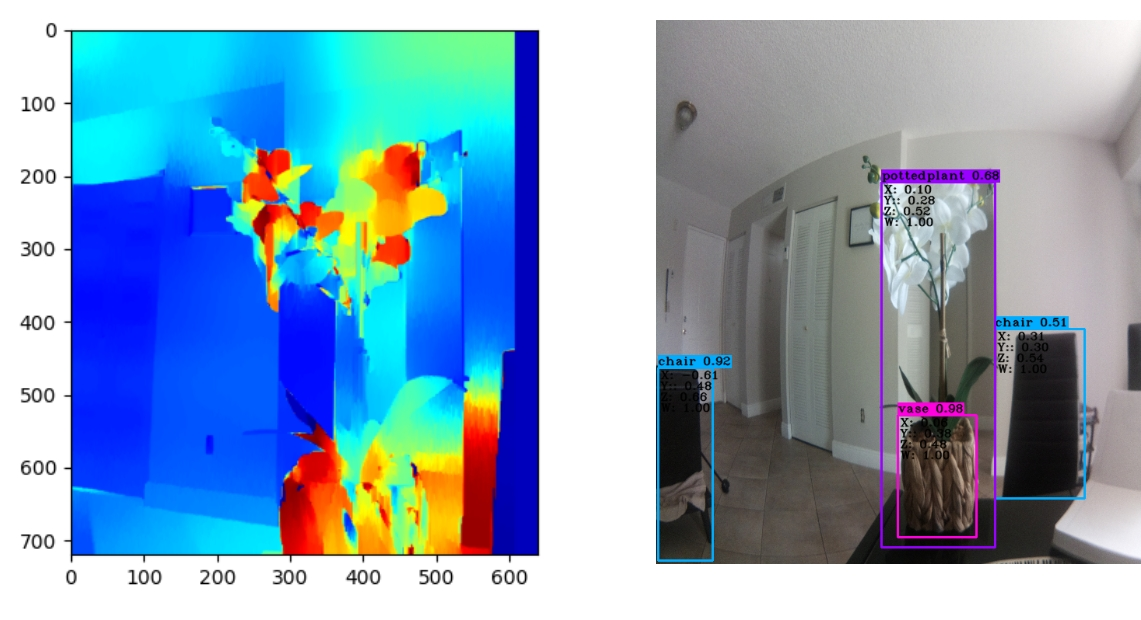
\includegraphics[scale=0.5]{Recursos/position_configuration_B.jpg}
    \caption[Mapa de disparidad y coordenadas con configuración B.]{Mapa de disparidad y coordenadas con configuración B. {\footnotesize Fuente: El Autor}}
    \label{pos_conf_B}
\end{figure}
El error absoluto del objeto para la configuración B es de 0.17
\begin{figure}[H]
    \centering
    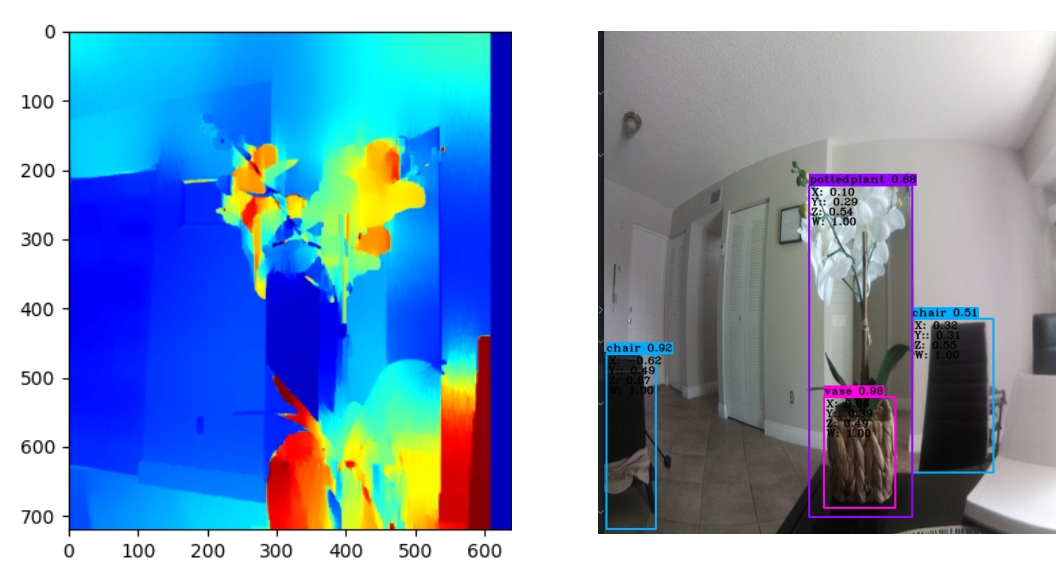
\includegraphics[scale=0.5]{Recursos/position_configuration_M.jpg}
    \caption[Mapa de disparidad y coordenadas con configuración M.]{Mapa de disparidad y coordenadas con configuración M. {\footnotesize Fuente: El Autor}}
    \label{pos_conf_M}
\end{figure}
El error absoluto del objeto para la configuración M es de 0.19.
\\
Por lo que el error absoluto promedio será de 0.18 m.
\section{Análisis de resultados}
Debido a que en la metodología seleccionada los píxeles son elegidos a partir de la imagen de entrada por el algoritmo de segmentación binaria, estos son iguales para todas las configuraciones, por lo que la posición varía conforme al mapa de disparidad. 
\\
En los 3 casos presentados se puede observar que sus mapas de disparidad son bastante similares y aunque el error es de 18 cm para objetos cercanos, a medida que un objeto se aleja superando 1 metro, la distancia mostrada no se encuentra bien representada, sin embargo estas tres configuraciones mantienen la relación de orden entre objetos de forma correcta, es decir; si un objeto se encuentra antes que otro este siempre tendrá una menor distancia en la coordenada Z.
\\
\\
El problema antes mencionado radica en que como se puede ver en la Figura \ref{disparity_with_postprocess} estos mapas de disparidad no tienen un paso gradual entre el rojo y el azul, además de que los píxeles más cercanos deberían reflejar un rojo más intenso (el rojo indica cercanía) esto se debe a que cuando se ajustaron los parámetros se buscó obtener un resultado que al menos respetara el orden entre objetos, por lo que para conseguir mejores resultados es menester tomar en cuenta un ajuste más preciso y que la imagen utilizada en dicho ajuste posea una mayor distinción de la profundidad, lo que se traduce en una mayor cantidad de objetos superpuestos y de ser posible una perspectiva que permita percibir mejor toda la profundidad de la escena. En cuanto a la velocidad sé probo el algoritmo con vídeo y este alcanzo en promedio 1.7 FPS en la máquina local, lo que implica que la rapidez se encuentra limitada únicamente por el modelo de reconocimiento, ya que el efecto del algoritmo estéreo es mínimo en comparación.